% ============================================================
%  CHAPITRE 7 : Dimensionnement théorique de l'évacuateur de crues
% ============================================================
\chapter{Dimensionnement théorique de l'évacuateur de crues}
\label{chap:dimensionnement_theorique}

% SECTION : INTRODUCTION
\section{Introduction}
\label{sec:intro_dimensionnement}

Avant d'entreprendre la modélisation numérique de l'évacuateur de crues du barrage Ahl Souss sous OpenFOAM, il est indispensable de disposer d'un cadre de référence théorique permettant à la fois de vérifier la cohérence du dimensionnement existant et de constituer une base de comparaison pour les résultats issus de la simulation 3D. Cette démarche correspond à la pratique courante de l'ingénierie hydraulique, où les méthodes analytiques classiques, les feuilles de calcul et les modèles 1D (HEC-RAS) sont systématiquement mobilisés en amont, voire en parallèle, des outils de simulation tridimensionnelle.

Ce chapitre reprend les données géométriques et hydrauliques du barrage Ahl Souss présentées au chapitre \ref{chap:barrage} et les exploite pour mener, étape par étape, le dimensionnement hydraulique complet de l'évacuateur de crues : vérification du profil du seuil déversant (section \ref{sec:profil_seuil}), établissement de la loi débit-charge (section \ref{sec:loi_debit_charge}), calcul de la courbe de remous le long du coursier (section \ref{sec:courbe_remous}), détermination de la hauteur des murs bajoyers à l'aide du logiciel HEC-RAS (section \ref{sec:murs_bajoyers}), vérification de la géométrie de la cuillère du saut de ski (section \ref{sec:geometrie_cuillere}), calcul de la distance d'impact du jet (section \ref{sec:distance_impact_jet}) et évaluation de l'affouillement à l'aval de l'ouvrage (section \ref{sec:affouillement}). L'ensemble de ces résultats est synthétisé en fin de chapitre (section \ref{sec:synthese_resultats_theoriques}) sous la forme d'un tableau récapitulatif qui servira de référence pour l'analyse comparative menée au chapitre \ref{chap:resultats_simulation}.

% SECTION : DONNÉES DE BASE ET HYPOTHÈSES DE CALCUL
\section{Données de base et hypothèses de calcul}
\label{sec:donnees_base_hypotheses}

Les calculs développés dans ce chapitre s'appuient sur les caractéristiques géométriques et hydrologiques du barrage Ahl Souss présentées au chapitre \ref{chap:barrage} : longueur déversante du seuil, cote de calage, charge de dimensionnement du profil, niveaux caractéristiques de la retenue (RN, NPHE), ainsi que sur les débits de pointe des crues de référence rappelés au tableau \ref{tab:debits_crues} (crues décennale, centennale, millénale et de période de retour 5\,000 ans).

Le tableau \ref{tab:donnees_base} synthétise l'ensemble des données d'entrée retenues pour les calculs des sections suivantes. Les valeurs reprises du chapitre \ref{chap:barrage} sont directement exploitables ; les paramètres complémentaires propres aux calculs hydrauliques du coursier (largeur, pente, coefficient de rugosité, cote du lit aval) seront précisés à partir des éléments topographiques et de la feuille de calcul Excel développée dans le cadre de cette étude.

\begin{table}[H]
    \centering
    \caption{Données géométriques et hydrauliques de base retenues pour le dimensionnement}
    \label{tab:donnees_base}
    \begin{tabular}{|l|c|c|}
        \hline
        \textbf{Paramètre} & \textbf{Symbole} & \textbf{Valeur retenue} \\
        \hline
        Longueur déversante du seuil & $L$ & 70 m \\
        \hline
        Cote du seuil déversant & $Z_s$ & 600,00 NGM \\
        \hline
        Charge de dimensionnement retenue pour la loi débit-charge (affinée) & $H_d$ & 3,07 m \\
        \hline
        Coefficient de débit de dimensionnement & $C_d$ & 2,15 \\
        \hline
        Hauteur du seuil au-dessus du radier aval & $P$ & 28 m \\
        \hline
        Charge maximale sous NPHE (note de calcul initiale) & $H_{NPHE}$ & 2,86 m \\
        \hline
        Débit évacué sous NPHE (note de calcul initiale) & $Q_{NPHE}$ & 730 m³/s \\
        \hline
        Débit évacué sous NPHEE (note de calcul initiale) & $Q_{NPHEE}$ & 1\,008 m³/s \\
        \hline
        Cote de calage du point bas de la cuillère (saut de ski) & $Z_c$ & 585,20 NGM \\
        \hline
        Rayon du bec déviateur & $R$ & 3 m \\
        \hline
        Angle de sortie du bec déviateur & $\theta$ & 40° \\
        \hline
        Largeur du coursier (en tête, $=L$) & $b$ & 70 m \\
        \hline
        Pente moyenne du coursier (talus aval) & $i$ & 1,25 m/m \\
        \hline
        Coefficient de rugosité (Manning-Strickler) & $K_s$ & 70 m$^{1/3}$/s \\
        \hline
        Cote du radier du bassin de dissipation & $Z_{aval}$ & 579,50 NGM \\
        \hline
    \end{tabular}
\end{table}

La longueur déversante $L = 70$ m est conforme à la note de calcul initiale de l'évacuateur de crues (chapitre \ref{chap:barrage}) et correspond à un seul déversoir (\textit{Nbr de passes} $= 1$) dans la feuille de calcul hydraulique développée pour la présente étude. Seule la charge de dimensionnement a été affinée par rapport à la note de calcul initiale : pour la géométrie du profil Creager (section \ref{sec:profil_seuil}), la charge de référence retenue est $H_{NPHE} = 2{,}86$ m, charge maximale sous NPHE de la note de calcul initiale (tableau \ref{tab:donnees_base}) ; pour la loi débit-charge (section \ref{sec:loi_debit_charge}), la feuille de calcul hydraulique développée pour la présente étude retient $H_d = 3{,}07$ m, au lieu de $H_d = 3{,}20$ m dans la note de calcul initiale. Les paramètres $C_d$, $P$, le coefficient de Strickler $K_s = 70$ m$^{1/3}$/s (béton lissé) et la pente moyenne du coursier $i = 0{,}80$ m/m (talus aval) sont issus directement de cette même feuille de calcul. La cote $Z_{aval} = 579{,}50$ NGM correspond au radier du bassin de dissipation défini au chapitre \ref{chap:barrage}.

\subsection{Débits de crue laminés retenus}
\label{subsec:debits_lamines}

Les débits de pointe $Q_p$ rappelés au tableau \ref{tab:debits_crues} correspondent aux débits entrant dans la retenue. Le débit effectivement évacué par l'évacuateur de crues, noté $Q_s$, est obtenu après laminage de l'hydrogramme de crue à travers la retenue du barrage Ahl Souss, à l'aide de la courbe hauteur-volume du réservoir et de la loi débit-charge du seuil déversant (section \ref{sec:loi_debit_charge}) : l'effet régulateur de la retenue se traduit par un débit évacué $Q_s$ inférieur au débit de pointe entrant $Q_p$, et par une charge $H$ sur le seuil correspondant à ce débit laminé. Le tableau \ref{tab:debits_lamines} présente les résultats de ce laminage pour les trois périodes de retour étudiées ; ce sont ces débits laminés $Q_s$ qui constituent la donnée d'entrée de l'ensemble des calculs hydrauliques développés dans la suite de ce chapitre.

\begin{table}[H]
    \centering
    \caption{Débits de crue laminés et charges correspondantes sur le seuil}
    \label{tab:debits_lamines}
    \begin{tabular}{|c|c|c|c|}
        \hline
        \textbf{Période de retour (ans)} & \textbf{$Q_p$ (m³/s)} & \textbf{$Q_s$ (m³/s)} & \textbf{$H$ (m)} \\
        \hline
        10 & 220 & 160,74 & 1,13 \\
        \hline
        100 & 520 & 507,54 & 2,32 \\
        \hline
        1\,000 & 820 & 794,93 & 3,07 \\
        \hline
    \end{tabular}
\end{table}

Les hypothèses générales suivantes sont adoptées pour l'ensemble des calculs théoriques de ce chapitre :
\begin{itemize}
    \item L'écoulement est traité en régime permanent pour chaque débit de crue considéré (approche quasi-stationnaire, indépendante de la phase de montée et de décrue de l'hydrogramme).
    \item Le fluide (eau) est supposé incompressible et à température constante.
    \item Les pertes de charge le long du coursier sont évaluées par la formule de Manning-Strickler.
    \item Les débits de crue laminés $Q_s$ du tableau \ref{tab:debits_lamines} (périodes de retour 10, 100 et 1\,000 ans) sont retenus comme scénarios de calcul, conformément à la campagne de simulations définie en introduction générale. La crue de période de retour 5\,000 ans (tableau \ref{tab:debits_crues}) n'a pas fait l'objet d'un laminage dans le cadre de la feuille de calcul hydraulique et n'est donc pas reprise dans le détail des calculs des sections suivantes.
    \item \textbf{La vidange de fond est négligée dans l'ensemble des calculs et de la modélisation numérique.} Le barrage Ahl Souss est équipé d'une vidange de fond composée de deux conduites en acier de diamètre 1\,000 mm, dont la capacité maximale sous retenue normale est de $12$ m³/s \cite{fiche_organes_restitution, note_calcul_vidange} (section \ref{sec:vidange_fond}). Cette valeur est négligeable devant les débits évacués par l'évacuateur de crues : elle représente respectivement $7{,}5\,\%$, $2{,}4\,\%$ et $1{,}5\,\%$ des débits laminés $Q_{10}$, $Q_{100}$ et $Q_{1000}$. Son influence sur le champ d'écoulement à la crête du seuil et le long du coursier est donc marginale. Par ailleurs, l'intégration de la vidange de fond dans la géométrie du modèle numérique OpenFOAM nécessiterait un maillage supplémentaire significatif et des conditions aux limites additionnelles, sans apporter de gain de précision perceptible sur les grandeurs d'intérêt (profil de la ligne d'eau, champ de vitesse sur le coursier, trajectoire du jet). Cette simplification est classique dans les études hydrauliques de ce type et ne compromet pas la validité des conclusions.
\end{itemize}

% SECTION : PROFIL DU SEUIL DÉVERSANT
\section{Profil du seuil déversant : vérification du profil Creager}
\label{sec:profil_seuil}

Le profil du seuil déversant est déterminé de manière à offrir la forme idéale pour une évacuation optimale, de telle sorte que la face inférieure de la lame déversante épouse constamment la surface du corps du barrage, évitant ainsi toute zone de dépression susceptible de provoquer de la cavitation. Dans cet objectif, l'ouvrage \textit{Design of Small Dams} de l'US Bureau of Reclamation \cite{usbr1987design} propose plusieurs familles de profils pour le seuil déversant ; la géométrie la plus couramment retenue, notamment au Maroc, est celle du profil Creager (ou profil WES).

\subsection{Forme du seuil déversoir}
\label{subsec:forme_seuil_deversoir}

La partie amont de ce profil est constituée de deux arcs de cercle, de rayons $R_1$ et $R_2$, déterminés à partir des abaques du \textit{Design of Small Dams}. La partie aval, de type Creager courbé, assure une évacuation optimale et son expression analytique adimensionnelle s'écrit \cite{usbr1987design} :

\begin{equation}
\frac{Y}{H_0} = -K \left(\frac{X}{H_0}\right)^{n}
\label{eq:creager_general_kn}
\end{equation}

avec :
\begin{itemize}
    \item $X$, $Y$ : coordonnées horizontale et verticale du profil, l'origine du repère étant prise à la crête du seuil, calée à la retenue normale (RN) ;
    \item $H_0$ : la charge de dimensionnement du profil, ici $H_0 = H_{NPHE} = 2{,}86$ m (tableau \ref{tab:donnees_base}) ;
    \item $K$, $n$ : des coefficients déterminés à partir des abaques du \textit{Design of Small Dams}, en fonction des rapports caractéristiques $h_a/H_0$ et $P/H_0$ ;
    \item $h_a$ : la charge de vitesse d'approche (hauteur cinétique de la charge d'eau au-dessus du seuil).
\end{itemize}

\subsubsection{Paramètres du projet}
\label{subsubsec:parametres_projet_creager}

Le tableau \ref{tab:parametres_creager} rappelle les grandeurs caractéristiques du projet utilisées pour la détermination du profil.

\begin{table}[H]
    \centering
    \caption{Données caractéristiques retenues pour la détermination du profil Creager}
    \label{tab:parametres_creager}
    \begin{tabular}{|l|c|c|}
        \hline
        \textbf{Paramètre} & \textbf{Symbole} & \textbf{Valeur} \\
        \hline
        Débit de laminage sous NPHE & $Q_{NPHE}$ & 730 m³/s \\
        \hline
        Longueur du seuil & $L$ & 70 m \\
        \hline
        Hauteur du seuil & $P$ & 28 m \\
        \hline
        Accélération de la pesanteur & $g$ & 9,81 m/s² \\
        \hline
        Charge de dimensionnement du profil & $H_0$ & 2,86 m \\
        \hline
    \end{tabular}
\end{table}

\subsubsection{Débit spécifique et vitesse d'approche}
\label{subsubsec:debit_specifique_vitesse}

Le débit spécifique (débit par mètre linéaire de seuil) sous $Q_{NPHE}$ vaut :

\begin{equation}
q = \frac{Q_{NPHE}}{L} = \frac{730}{70} \approx 10{,}4286 \text{ m}^3/\text{s/m}
\label{eq:debit_specifique_usace}
\end{equation}

La vitesse d'approche, calculée en considérant la section d'écoulement amont de hauteur $(P+H_0)$ et de largeur $L$, vaut :

\begin{equation}
V = \frac{Q_{NPHE}}{(P+H_0) \cdot L} = \frac{730}{(28+2{,}86)\times 70} \approx 0{,}1142 \text{ m/s}
\label{eq:vitesse_approche_usace}
\end{equation}

La charge de vitesse d'approche (hauteur d'approche) correspondante est :

\begin{equation}
h_a = \frac{V^2}{2g} = \frac{0{,}1142^2}{2\times 9{,}81} \approx 0{,}00582 \text{ m}
\label{eq:charge_vitesse_approche}
\end{equation}

\subsubsection{Rapports caractéristiques pour la lecture des abaques}
\label{subsubsec:rapports_caracteristiques}

Les abaques du \textit{Design of Small Dams} sont entrés avec les deux rapports adimensionnels suivants :

\begin{equation}
\frac{h_a}{H_0} = \frac{0{,}00582}{2{,}86} \approx 0{,}00204
\label{eq:rapport_ha_hnphe}
\end{equation}

\begin{equation}
\frac{P}{H_0} = \frac{28}{2{,}86} \approx 9{,}79
\label{eq:rapport_p_hnphe}
\end{equation}

\subsubsection{Coefficients $K$ et $n$ du profil aval}
\label{subsubsec:coeffs_kn_usace}

\begin{figure}[H]
    \centering
    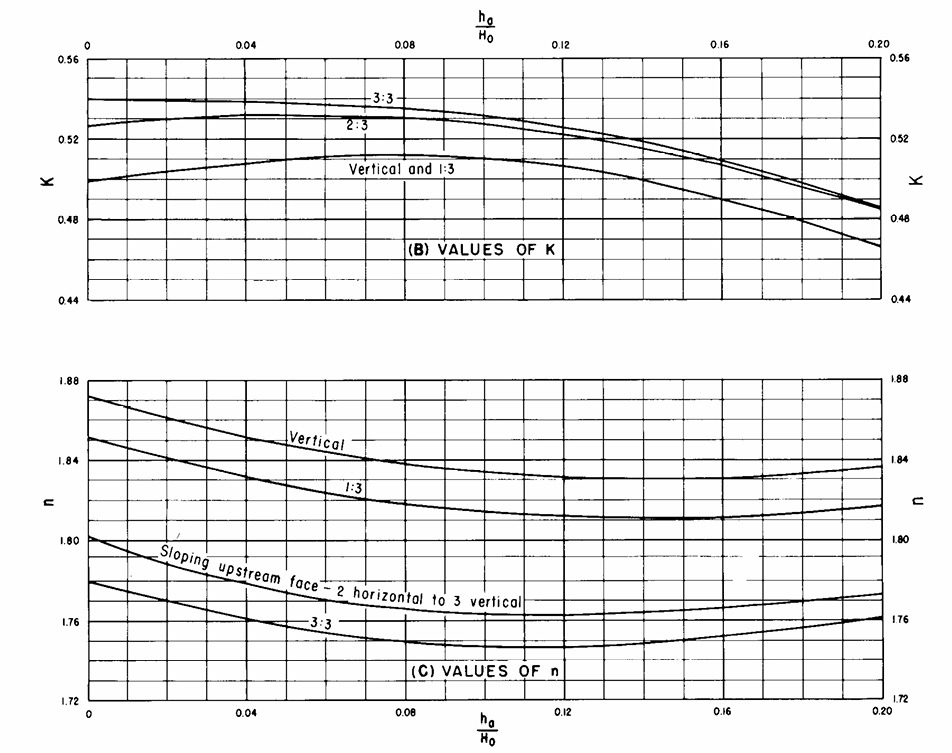
\includegraphics[width=0.85\textwidth]{figures/abaque_kn.jpg}
    \caption{Abaque de détermination des coefficients $K$ et $n$ du profil aval, en fonction de $h_a/H_0$ et de l'inclinaison du parement amont (figure 9-21 -- \textit{Factors for definition of nappe-shaped crest profiles}, planche 288-D-2406, \cite{usbr1987design}).}
    \label{fig:abaque_kn}
\end{figure}

Pour un parement amont vertical, avec $h_a/H_0 \approx 0{,}00204$ et $P/H_0 \approx 9{,}79$, la lecture de l'abaque (figure \ref{fig:abaque_kn}) donne :

\begin{equation}
K = 0{,}5 \qquad n = 1{,}872
\label{eq:coeffs_kn_usace}
\end{equation}

Le tableau \ref{tab:coeffs_kn_creager} récapitule ces deux coefficients.

\begin{table}[H]
    \centering
    \caption{Coefficients $K$ et $n$ du profil Creager}
    \label{tab:coeffs_kn_creager}
    \begin{tabular}{|c|c|c|}
        \hline
        \textbf{Coefficient} & \textbf{Valeur} & \textbf{Unité} \\
        \hline
        $K$ & 0,5 & sans dimension \\
        \hline
        $n$ & 1,872 & sans dimension \\
        \hline
    \end{tabular}
\end{table}

\subsubsection{Coordonnées du point de raccordement seuil-coursier $(X_c,Y_c)$}
\label{subsubsec:coord_xc_yc}

\begin{figure}[H]
    \centering
    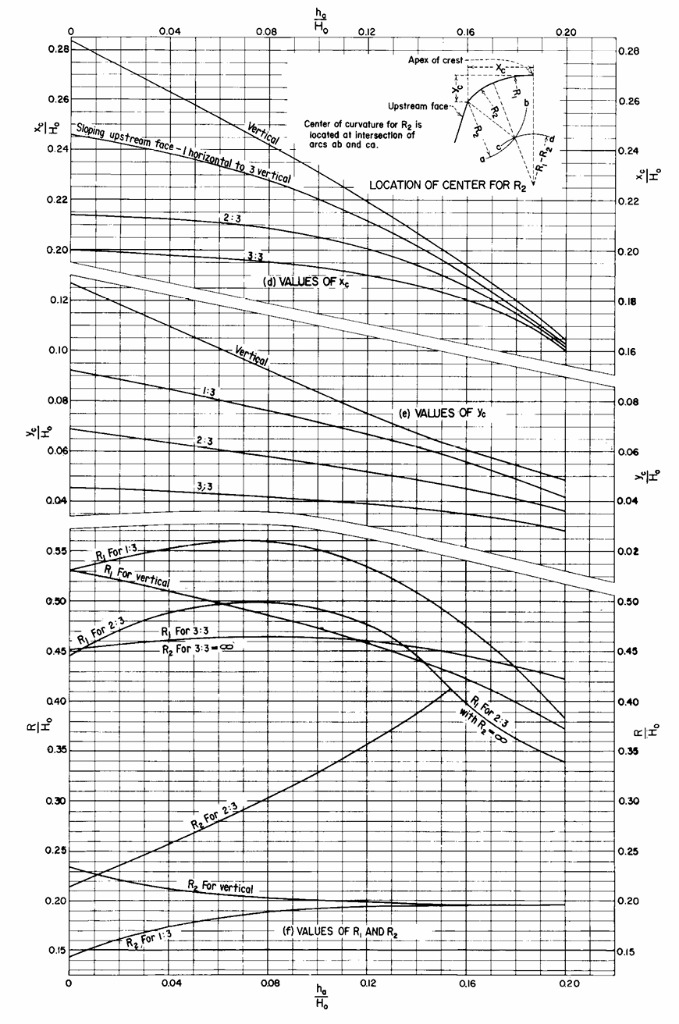
\includegraphics[width=0.85\textwidth]{figures/abaque_Xc_Yc.jpeg}
    \caption{Les paramètres caractéristiques de la partie amont du profil Creager (figure 9-21 -- \textit{Factors for definition of nappe-shaped crest profiles}, planche 288-D-2407, \cite{usbr1987design}).}
    \label{fig:abaque_xc_yc}
\end{figure}

D'après l'abaque (figure \ref{fig:abaque_xc_yc}), pour un parement amont vertical :

\begin{equation}
\frac{X_c}{H_0} = 0{,}283 \;\Rightarrow\; X_c = 0{,}283 \times 2{,}86 \approx 0{,}80652 \text{ m}
\label{eq:coord_xc}
\end{equation}

\begin{equation}
\frac{Y_c}{H_0} = 0{,}126 \;\Rightarrow\; Y_c = 0{,}126 \times 2{,}86 \approx 0{,}3603 \text{ m}
\label{eq:coord_yc}
\end{equation}

\subsubsection{Rayons de raccordement amont et aval $R_1$, $R_2$}
\label{subsubsec:rayons_r1_r2}

D'après l'abaque (figure \ref{fig:abaque_xc_yc}) :

\begin{equation}
\frac{R_1}{H_0} = 0{,}53 \;\Rightarrow\; R_1 = 0{,}53 \times 2{,}86 \approx 1{,}51 \text{ m}
\label{eq:rayon_r1}
\end{equation}

\begin{equation}
\frac{R_2}{H_0} = 0{,}233 \;\Rightarrow\; R_2 = 0{,}233 \times 2{,}86 \approx 0{,}6721 \text{ m}
\label{eq:rayon_r2}
\end{equation}

\subsubsection{Tableau récapitulatif des paramètres du seuil}
\label{subsubsec:recap_profil_usace}

Le tableau \ref{tab:recap_profil_usace} récapitule l'ensemble des paramètres géométriques ainsi obtenus.

\begin{table}[H]
    \centering
    \caption{Récapitulatif des paramètres géométriques du profil Creager ($H_0=2{,}86$ m)}
    \label{tab:recap_profil_usace}
    \begin{tabular}{|c|c|c|c|}
        \hline
        \textbf{Paramètre} & \textbf{Rapport} & \textbf{Valeur du rapport} & \textbf{Valeur (m)} \\
        \hline
        $X_c$ & $X_c/H_0$ & 0,283 & 0,80652 \\
        \hline
        $Y_c$ & $Y_c/H_0$ & 0,126 & 0,3603 \\
        \hline
        $R_1$ & $R_1/H_0$ & 0,53 & 1,51 \\
        \hline
        $R_2$ & $R_2/H_0$ & 0,233 & 0,6721 \\
        \hline
    \end{tabular}
\end{table}

\subsubsection{Équation du profil retenu}
\label{subsubsec:equation_profil_usace}

Avec les coefficients $K=0{,}5$ et $n=1{,}872$ (équation \ref{eq:coeffs_kn_usace}), le profil aval s'écrit, sous forme adimensionnelle (équation \ref{eq:creager_general_kn}) :

\begin{equation}
\frac{Y}{H_0} = -0{,}5 \left(\frac{X}{H_0}\right)^{1{,}872}
\label{eq:profil_creager_hnphe_forme}
\end{equation}

soit, numériquement, avec $H_0=2{,}86$ m :

\begin{equation}
Y = -0{,}5 \times 2{,}86 \times \left(\frac{X}{2{,}86}\right)^{1{,}872} = -1{,}43 \left(\frac{X}{2{,}86}\right)^{1{,}872}
\label{eq:profil_creager_hnphe}
\end{equation}

Le signe négatif de l'équation \ref{eq:profil_creager_hnphe} correspond à un axe $Y$ orienté vers le haut, l'origine étant prise à la crête du seuil ($X=Y=0$) : les points du profil, situés sous la crête, ont donc une ordonnée $Y<0$. L'équation \ref{eq:profil_creager_hnphe} est valable depuis la crête ($X=0$) jusqu'au point de raccordement avec le coursier $(X_c,Y_c) = (0{,}80652\,;\,0{,}3603)$ m (équations \ref{eq:coord_xc}-\ref{eq:coord_yc}).

\subsubsection{Tableau de points pour le tracé de la courbe}
\label{subsubsec:points_profil_usace}

Pour un tracé précis de la courbe, le tableau \ref{tab:points_profil_creager_hnphe} fournit les coordonnées $(X,Y)$ calculées par l'équation \ref{eq:profil_creager_hnphe}, pour $X$ variant de 0 à 2,8 m par pas de 0,1 m, soit l'intervalle couvrant le seuil jusqu'au-delà du point de raccordement $X_c=0{,}80652$ m.

\begin{table}[H]
    \centering
    \caption{Points de la courbe du profil Creager ($H_0=2{,}86$ m, équation \ref{eq:profil_creager_hnphe})}
    \label{tab:points_profil_creager_hnphe}
    \begin{tabular}{|c|c||c|c||c|c|}
        \hline
        \textbf{$X$ (m)} & \textbf{$Y$ (m)} & \textbf{$X$ (m)} & \textbf{$Y$ (m)} & \textbf{$X$ (m)} & \textbf{$Y$ (m)} \\
        \hline
        0 & 0 & 1,0 & -0,20000000 & 2,0 & -0,73207933 \\
        \hline
        0,1 & -0,00268553 & 1,1 & -0,23906561 & 2,1 & -0,80209261 \\
        \hline
        0,2 & -0,00983010 & 1,2 & -0,28135672 & 2,2 & -0,87507495 \\
        \hline
        0,3 & -0,02099911 & 1,3 & -0,32683755 & 2,3 & -0,95100873 \\
        \hline
        0,4 & -0,03598208 & 1,4 & -0,37547556 & 2,4 & -1,02987719 \\
        \hline
        0,5 & -0,05463889 & 1,5 & -0,42724091 & 2,5 & -1,11166438 \\
        \hline
        0,6 & -0,07686509 & 1,6 & -0,48210607 & 2,6 & -1,19635509 \\
        \hline
        0,7 & -0,10257783 & 1,7 & -0,54004553 & 2,7 & -1,28393478 \\
        \hline
        0,8 & -0,13170870 & 1,8 & -0,60103550 & 2,8 & -1,37438951 \\
        \hline
        0,9 & -0,16419955 & 1,9 & -0,66505373 & & \\
        \hline
    \end{tabular}
\end{table}

\subsection{Tracé géométrique du profil sous AutoCAD}
\label{subsec:trace_autocad}

Le tracé du profil de l'évacuateur sous AutoCAD est mené à partir des résultats des calculs théoriques, selon la méthodologie en quatre étapes successives suivante :
\begin{enumerate}
    \item \textbf{Tracé des deux cercles de raccordement amont et aval ($R_1$ et $R_2$)} : La partie amont du profil comprend deux arcs de cercle. Le rayon amont $R_1 = 1{,}51$ m assure le raccordement tangentiel entre le parement amont vertical et la crête du seuil. Le rayon aval $R_2 = 0{,}6721$ m assure le raccordement entre la crête et le début du profil parabolique Creager.
    \item \textbf{Tracé du seuil de l'évacuateur} : Le seuil est tracé point par point à partir de l'équation parabolique adimensionnelle du profil Creager (équation \ref{eq:profil_creager_hnphe}) et des coordonnées définies (tableau \ref{tab:points_profil_creager_hnphe}). Ce tracé s'étend depuis la crête ($X=0, Y=0$) jusqu'au point de raccordement avec le coursier $(X_c,Y_c) = (0{,}80652\,;\,0{,}3603)$ m.
    \item \textbf{Tracé du coursier (partie rectiligne)} : Le coursier est une ligne droite débutant au point de raccordement $(X_c,Y_c)$ avec une pente de $0{,}8$ H pour $1$ V (angle d'inclinaison par rapport à l'horizontale $\alpha \approx 51{,}34^\circ$).
    L'angle d'inclinaison est obtenu par :
    \begin{equation}
    \alpha = \arctan\left(\frac{1}{0{,}8}\right) \approx 51{,}34^\circ
    \label{eq:angle_coursier}
    \end{equation}
    L'équation de cette droite s'écrit :
    \begin{equation}
    Y = 1{,}25\,X - 0{,}64785
    \label{eq:droite_coursier}
    \end{equation}
    Le coursier se prolonge vers l'aval jusqu'au départ de la cuillère, à la cote $586{,}54$ m.
    \item \textbf{Tracé de la cuillère de dissipation (saut de ski)} : La cuillère débute à la cote $586{,}54$ m et se compose d'un arc de cercle de rayon $R_3 = 3$ m se terminant avec un angle de sortie de $\beta = 40^\circ$ orienté vers le haut, le point le plus bas étant calé à la cote de calage de référence $Z_c = 585{,}20$ NGM.
\end{enumerate}

Le tableau \ref{tab:recap_trace_autocad} récapitule l'ensemble des cotes et paramètres géométriques appliqués pour ce tracé géométrique.

\begin{table}[H]
    \centering
    \caption{Récapitulatif des paramètres pour le tracé du profil sous AutoCAD}
    \label{tab:recap_trace_autocad}
    \begin{tabular}{|l|c|c|}
        \hline
        \textbf{Élément} & \textbf{Paramètre} & \textbf{Valeur} \\
        \hline
        Rayon amont & $R_1$ & 1,51 m \\
        \hline
        Rayon aval & $R_2$ & 0,6721 m \\
        \hline
        Point de raccordement (début coursier) & $X_c$ & 0,80652 m \\
        \hline
        Point de raccordement (début coursier) & $Y_c$ & 0,3603 m \\
        \hline
        Équation du seuil & $Y=f(X)$ & $Y=-1{,}43\,(X/2{,}86)^{1{,}872}$ \\
        \hline
        Pente du coursier & $i$ & 0,8 H/V \\
        \hline
        Angle du coursier & $\alpha$ & $\arctan(1{,}25)\approx 51{,}34^\circ$ \\
        \hline
        Équation du coursier & $Y=1{,}25X-0{,}64785$ & -- \\
        \hline
        Début de la cuillère & Cote & 586,54 m \\
        \hline
        Rayon de la cuillère & $R_3$ & 3 m \\
        \hline
        Angle de sortie de la cuillère & $\beta$ & 40° \\
        \hline
    \end{tabular}
\end{table}

La figure \ref{fig:autocad_profil_complet} illustre le tracé géométrique finalisé du profil Creager de l'évacuateur de crues tracé sous AutoCAD avec ses dimensions principales.

\begin{figure}[H]
    \centering
    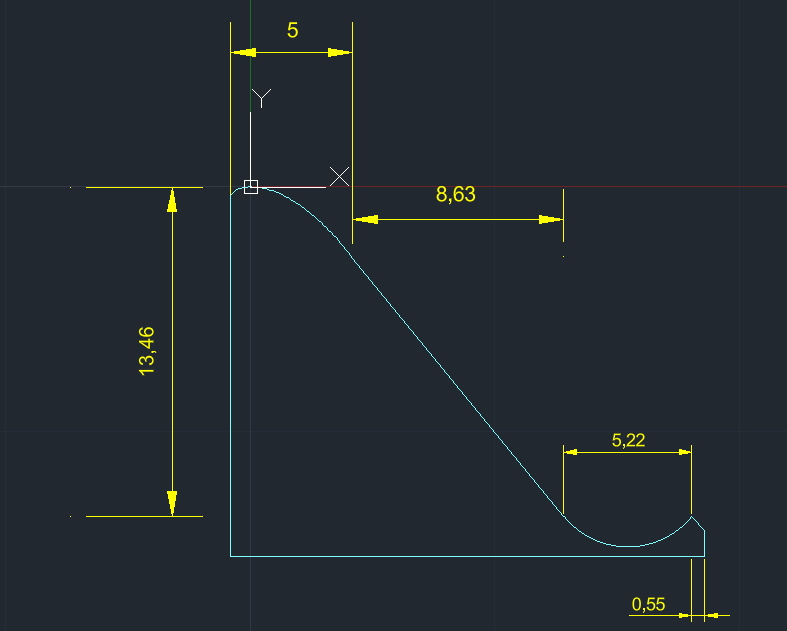
\includegraphics[width=0.85\textwidth]{figures/profil_autocad.png}
    \caption{Tracé géométrique final du profil Creager de l'évacuateur de crues sous AutoCAD avec ses dimensions principales (en mètres).}
    \label{fig:autocad_profil_complet}
\end{figure}

\subsection{La courbe du profil Creager}
\label{subsec:courbe_profil_creager}

La figure \ref{fig:profil_creager} présente la courbe du profil Creager obtenue par application de l'équation \ref{eq:profil_creager_hnphe} (tableau \ref{tab:points_profil_creager_hnphe}), exprimée en cote du radier (NGM). La cote du radier représentée s'en déduit par $\text{Cote} = Z_s + Y$, avec $Z_s = 600{,}00$ NGM (tableau \ref{tab:donnees_base}).

\begin{figure}[H]
    \centering
    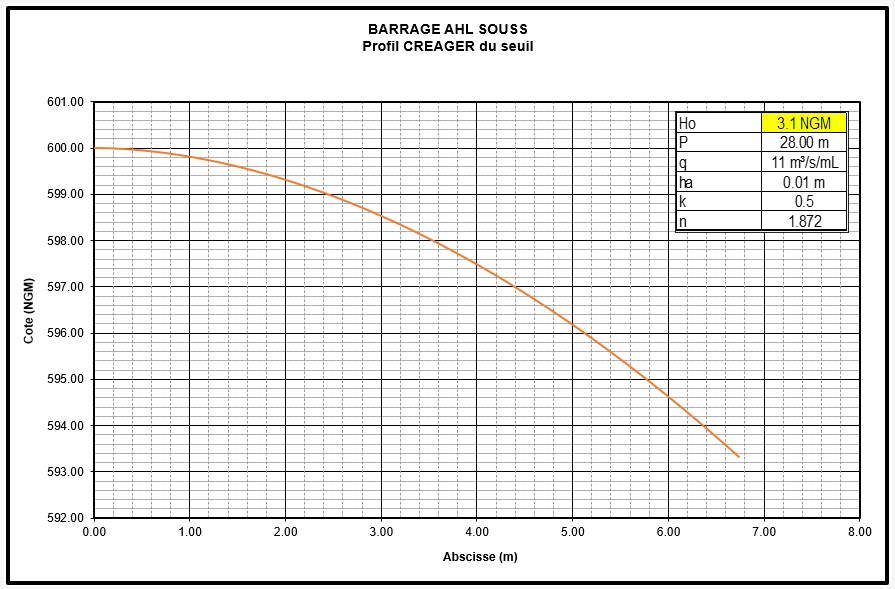
\includegraphics[width=0.85\textwidth]{figures/courbe_profil_creager.png}
    \caption{Courbe du profil Creager de l'évacuateur de crues (origine des abscisses $X=0$ au sommet du seuil ; axe vertical en cote du radier, NGM, décroissante vers l'aval du profil).}
    \label{fig:profil_creager}
\end{figure}



% SECTION : LOI DÉBIT-CHARGE
\section{Loi débit-charge et capacité d'évacuation du seuil}
\label{sec:loi_debit_charge}

La relation générale entre le débit déversé $Q$ et la charge $H$ au-dessus d'un seuil de type Creager s'écrit \cite{usbr1987design, chow1959open} :

\begin{equation}
Q = C \cdot L \cdot H^{3/2}
\label{eq:debit_seuil}
\end{equation}

où $C$ est le coefficient de débit, $L = 70$ m la longueur déversante du seuil (tableau \ref{tab:donnees_base}) et $H$ la charge mesurée au-dessus de la cote du seuil ($Z_s = 600{,}00$ NGM).

Le coefficient $C$ n'est pas constant : il dépend du rapport $H/H_d$ entre la charge effective et la charge de dimensionnement, selon des abaques établis expérimentalement par l'USBR \cite{usbr1987design}. Pour $H = H_d$, $C$ atteint sa valeur de dimensionnement $C_d = 2{,}15$ (tableau \ref{tab:donnees_base}) ; pour $H < H_d$, $C$ est légèrement inférieur à $C_d$ ; pour $H > H_d$, $C$ peut légèrement le dépasser.

\textbf{Vérification à partir des données NPHE.} En exploitant les valeurs de charge et de débit sous NPHE données au chapitre \ref{chap:barrage} ($H_{NPHE} = 2{,}86$ m pour $Q_{NPHE} = 730$ m³/s, soit $H_{NPHE}/H_d \approx 2{,}86/3{,}0677 \approx 0{,}93$), le coefficient de débit correspondant vaut :

\begin{equation}
C = \frac{Q_{NPHE}}{L \cdot H_{NPHE}^{3/2}} = \frac{730}{70 \times 2{,}86^{1,5}} \approx 2{,}16
\label{eq:coeff_debit_verif}
\end{equation}

Cette valeur est très proche du coefficient de dimensionnement $C_d = 2{,}15$ retenu pour la présente étude, l'écart résiduel s'expliquant par le fait que $Q_{NPHE}$ et $H_{NPHE}$ proviennent de la note de calcul initiale (chapitre \ref{chap:barrage}) tandis que $L$ et $H_d$ correspondent aux valeurs affinées de la présente étude. Cette concordance confirme la validité de la loi débit-charge retenue.

\textbf{Détermination de la charge pour chaque débit de crue.} La charge $H$ correspondant à chacun des débits laminés retenus (tableau \ref{tab:debits_lamines}) est obtenue par résolution itérative de l'équation \ref{eq:debit_seuil}, le coefficient $C$ dépendant lui-même de $H$ via le rapport $H/H_d$ (procédure de calcul implémentée dans la feuille de calcul développée pour cette étude) :
\begin{enumerate}
    \item Initialiser $C = C_d$ (valeur de dimensionnement) ;
    \item Calculer $H = (Q / (C \cdot L))^{2/3}$ ;
    \item Mettre à jour $C$ à partir du rapport $H/H_d$ et de l'abaque USBR ;
    \item Répéter les étapes 2 et 3 jusqu'à convergence.
\end{enumerate}

Les résultats de cette procédure sont reportés dans le tableau \ref{tab:loi_debit_charge} et représentés graphiquement à la figure \ref{fig:courbe_debit_charge}.

\begin{table}[H]
    \centering
    \caption{Loi débit-charge du seuil déversant pour les débits laminés retenus}
    \label{tab:loi_debit_charge}
    \begin{tabular}{|c|c|c|c|c|c|}
        \hline
        \textbf{Période de retour (ans)} & \textbf{$Q$ (m³/s)} & \textbf{$H/H_d$} & \textbf{$C/C_d$} & \textbf{$C$} & \textbf{$H$ (m)} \\
        \hline
        10 & 160,74 & 0,369 & 0,893 & 1,92 & 1,13 \\
        \hline
        100 & 507,54 & 0,756 & 0,969 & 2,08 & 2,32 \\
        \hline
        1\,000 & 794,93 & 1,000 & 1,001 & 2,15 & 3,07 \\
        \hline
    \end{tabular}
\end{table}

\begin{figure}[H]
    \centering
    \begin{tikzpicture}
    \begin{axis}[
        width=0.85\textwidth,
        height=7cm,
        xlabel={$H$ (m)},
        ylabel={$Q$ (m\textsuperscript{3}/s)},
        grid=major,
        legend pos=north west,
        legend style={font=\small},
    ]
    \addplot[thick, blue] table[x=H,y=Q] {data/evc_qh.dat};
    \addlegendentry{Loi débit-charge $Q=f(H)$}
    \addplot[only marks, mark=*, mark size=2.5pt, red] coordinates {(1.13183498225396,160.735240718924) (2.31784974886398,507.535888342577) (3.06731336836435,794.925467002904)};
    \addlegendentry{$Q_{10}$, $Q_{100}$, $Q_{1000}$}
    \end{axis}
    \end{tikzpicture}
    \caption{Courbe débit-charge du seuil déversant de l'évacuateur de crues, avec les points correspondant aux trois débits laminés retenus.}
    \label{fig:courbe_debit_charge}
\end{figure}

% SECTION : COURBE DE REMOUS
\section{Calcul de la courbe de remous sur le coursier}
\label{sec:courbe_remous}

\subsection{Principe de la méthode pas-à-pas}
\label{subsec:principe_methode_pas_a_pas}

Le coursier de l'évacuateur de crues est un canal à forte pente sur lequel l'écoulement, critique au voisinage de la crête du seuil, devient rapidement torrentiel (régime supercritique). La détermination du profil de la ligne d'eau le long du coursier relève du calcul des écoulements graduellement variés, régi par l'équation différentielle \cite{chow1959open} :

\begin{equation}
\frac{dy}{dx} = \frac{S_0 - S_f}{1 - Fr^2}
\label{eq:gvf}
\end{equation}

où $y$ est la profondeur d'écoulement, $x$ l'abscisse le long du coursier, $S_0$ la pente du radier, $S_f$ la pente de la ligne d'énergie (perte de charge unitaire) et $Fr$ le nombre de Froude, défini par :

\begin{equation}
Fr = \frac{V}{\sqrt{g \, y}}
\label{eq:froude}
\end{equation}

La pente de frottement $S_f$ (pente de la ligne d'énergie) est évaluée à l'aide de la formule de Manning-Strickler :

\begin{equation}
S_f = \left(\frac{V}{K_s \, R_h^{2/3}}\right)^2
\label{eq:manning_strickler}
\end{equation}

avec $V$ la vitesse moyenne, $R_h$ le rayon hydraulique et $K_s$ le coefficient de Strickler du coursier, pris égal à $K_s = 70$ m$^{1/3}$/s pour un coursier en béton lisse (tableau \ref{tab:donnees_base}).

\subsection{Application au coursier de l'évacuateur de crues}
\label{subsec:application_courbe_remous}

La méthode pas-à-pas (ou méthode par tronçons) consiste à discrétiser le coursier en une succession de sections espacées d'un pas $\Delta x$, et à appliquer entre deux sections consécutives $i$ et $i+1$ l'équation de l'énergie :

\begin{equation}
Z_i + y_i + \frac{V_i^2}{2g} = Z_{i+1} + y_{i+1} + \frac{V_{i+1}^2}{2g} + \overline{S_f}\,\Delta x
\label{eq:energie_pas_a_pas}
\end{equation}

où $Z_i$ désigne la cote du radier à la section $i$ et $\overline{S_f}$ la pente de perte de charge moyenne entre les sections $i$ et $i+1$.

Le calcul est initialisé à la crête du seuil, où la profondeur correspond à la profondeur critique associée au débit considéré, puis mené de proche en proche vers l'aval (le calcul en régime supercritique progresse naturellement depuis l'amont vers l'aval). Cette procédure a été implémentée dans une feuille de calcul, pour chacun des trois débits laminés retenus (tableau \ref{tab:debits_lamines}).

Cette procédure fournit, pour chacun des trois débits laminés étudiés, l'ensemble des points $(x, Z, y, V, E, Fr)$ le long du coursier ; le détail de ces résultats est reporté en annexe, et l'ensemble des points calculés sert à tracer les profils de la figure \ref{fig:profil_ligne_eau}.

\begin{figure}[H]
    \centering
    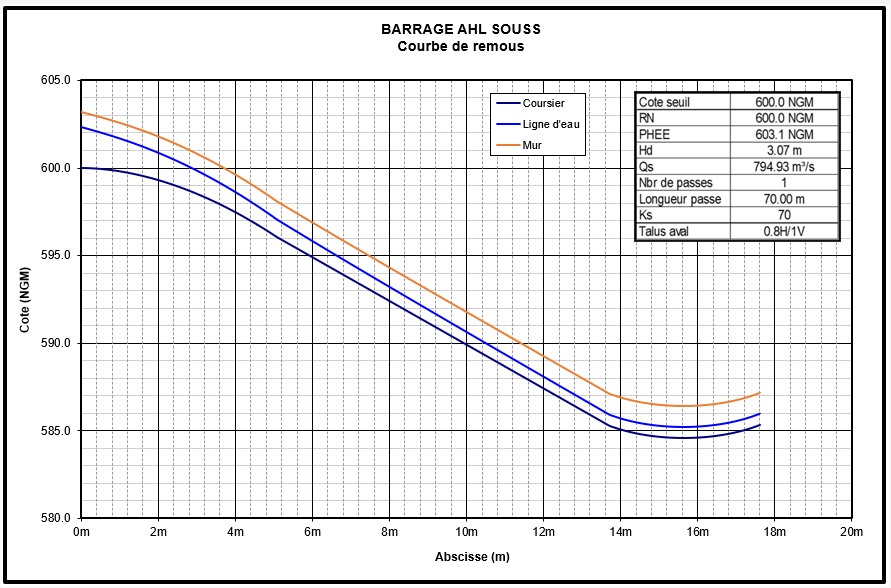
\includegraphics[width=0.85\textwidth]{figures/courbe_remous.png}
    \caption{Courbe de remous calculée par la méthode pas-à-pas, depuis la crête du seuil, pour le débit millénal laminé $Q_{1000} = 794{,}93$ m³/s : profil du radier, ligne d'eau et hauteur du mur bajoyer.}
    \label{fig:profil_ligne_eau}
\end{figure}

% SECTION : HAUTEUR DES MURS BAJOYERS
\section{Détermination de la hauteur des murs bajoyers}
\label{sec:murs_bajoyers}

\subsection{Présentation de l'outil HEC-RAS}
\label{subsec:presentation_hecras}

HEC-RAS (\textit{Hydrologic Engineering Center -- River Analysis System}) est un logiciel développé par le \textit{US Army Corps of Engineers}, largement utilisé en ingénierie hydraulique pour la modélisation unidimensionnelle (1D) et bidimensionnelle (2D) des écoulements à surface libre \cite{usace2016hecras}. Il permet de calculer le profil de la ligne d'eau en régime permanent (\textit{Steady Flow Analysis}) ou transitoire (\textit{Unsteady Flow Analysis}) le long d'un cours d'eau ou d'un ouvrage hydraulique, à partir d'une géométrie définie par une succession de sections transversales.

Le moteur de calcul de HEC-RAS repose sur la méthode du pas-à-pas standard (\textit{standard step method}), fondée sur la même équation de l'énergie que celle présentée à la section \ref{sec:courbe_remous} \cite{usace2016hecras, chow1959open}. Il est capable de traiter les régimes fluvial, torrentiel et mixte, ce qui le rend particulièrement adapté à l'étude des coursiers d'évacuateurs de crues, où l'écoulement transite du régime critique (à la crête) au régime torrentiel (sur le coursier).

Dans le cadre de cette étude, HEC-RAS est utilisé pour modéliser l'écoulement le long du coursier de l'évacuateur de crues et fournir, pour chaque débit de crue, le profil de la ligne d'eau servant de base à la détermination de la hauteur des murs bajoyers. Les résultats de cette modélisation 1D constituent également un second élément de comparaison avec les résultats de la modélisation OpenFOAM (chapitre \ref{chap:resultats_simulation}), en complément de la méthode pas-à-pas sous Excel (section \ref{sec:courbe_remous}).

\subsection{Modélisation 1D du coursier sous HEC-RAS}
\label{subsec:modelisation_hecras}

La géométrie du coursier a été introduite dans HEC-RAS sous la forme d'une succession de sections transversales (\textit{cross-sections}), espacées régulièrement le long de l'axe d'écoulement et établies à partir du profil type de l'ouvrage (profil AutoCAD / SketchUp, cf. section \ref{sec:sketchup}). Pour chaque section, les paramètres suivants ont été renseignés :
\begin{itemize}
    \item La géométrie transversale (largeur du coursier $b$ et géométrie des murs bajoyers) ;
    \item La cote du radier $Z$, déduite du profil Creager (section \ref{sec:profil_seuil}) puis de la pente du coursier ;
    \item Le coefficient de rugosité de Manning $n$, associé à la nature du revêtement en béton du coursier.
\end{itemize}

Le régime d'écoulement étant torrentiel sur l'ensemble du coursier, la condition aux limites amont est fixée à la profondeur critique au niveau de la crête du seuil, et le calcul est mené en régime \textit{supercritique} (option \textit{Mixed} de HEC-RAS, qui permet de basculer automatiquement entre régimes si nécessaire). Une analyse en régime permanent (\textit{Steady Flow Analysis}) est réalisée séparément pour chacun des trois débits laminés retenus (tableau \ref{tab:debits_lamines}), ce qui permet d'obtenir, pour chaque débit, le profil complet de la ligne d'eau le long du coursier.

\begin{figure}[H]
    \centering
    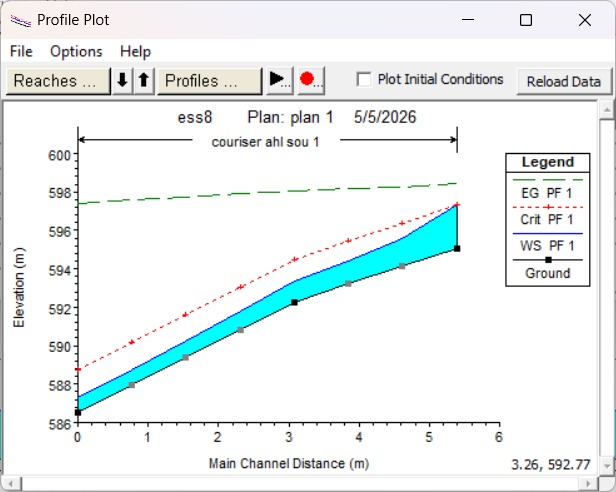
\includegraphics[width=0.6\textwidth]{figures/hecras_profile_plot.jpeg}
    \caption{Profil en long de la ligne d'eau du coursier obtenu sous HEC-RAS (\textit{Profile Plot}) : profil du radier (\textit{Ground}), ligne d'eau (\textit{WS PF 1}) et ligne d'énergie (\textit{EG PF 1}).}
    \label{fig:hecras_profil}
\end{figure}

\subsection{Hauteur des murs bajoyers retenue}
\label{subsec:hauteur_murs_retenue}

La hauteur des murs bajoyers $H_{mur}$ doit permettre de contenir la lame d'eau en écoulement sur le coursier, tout en intégrant une revanche $R_v$ destinée à couvrir les phénomènes non pris en compte par le calcul 1D (entraînement d'air et foisonnement de la lame d'eau, vagues et ondes de choc obliques, incertitudes sur la rugosité) :

\begin{equation}
H_{mur} = y_{max} + R_v
\label{eq:hauteur_mur}
\end{equation}

où $y_{max}$ est la profondeur d'eau maximale le long du coursier pour le débit considéré, obtenue par la méthode pas-à-pas (section \ref{sec:courbe_remous}) et confirmée par la modélisation HEC-RAS. Dans les trois cas étudiés, la profondeur maximale est obtenue dès la crête du seuil ($X=0$), où la lame d'eau est encore peu accélérée, avant de diminuer rapidement le long du coursier (figure \ref{fig:profil_ligne_eau}).

\subsubsection{Calcul de la revanche $R_v$}
\label{subsubsec:calcul_revanche}

La revanche $R_v$ est destinée à couvrir les phénomènes non pris en compte par le calcul 1D (entraînement d'air et foisonnement de la lame d'eau, vagues et ondes de choc obliques, incertitudes sur la rugosité). Elle est calculée, dans la feuille de calcul, à l'aide de la formule empirique suivante \cite{usbr1987design}, fonction de la vitesse moyenne $V$ et de la profondeur d'écoulement $y$ au point de hauteur maximale (crête du seuil, $X=0$) :

\begin{equation}
R_v = 0{,}61 + 0{,}037 \, V \, y^{1/3}
\label{eq:revanche}
\end{equation}

avec $V$ en m/s et $y$ en m. Cette relation traduit l'augmentation de la revanche avec la vitesse d'écoulement : plus le coursier est rapide, plus l'entraînement d'air et le foisonnement de la lame d'eau sont importants, et plus la revanche nécessaire est grande. Le tableau \ref{tab:revanche} présente, pour chacun des trois débits laminés retenus, les valeurs de $V$ et $y$ au point de hauteur maximale ainsi que la revanche $R_v$ qui en résulte.

\begin{table}[H]
    \centering
    \caption{Calcul de la revanche $R_v$ au point de hauteur maximale (crête du seuil)}
    \label{tab:revanche}
    \begin{tabular}{|c|c|c|c|c|}
        \hline
        \textbf{Période de retour (ans)} & \textbf{$Q$ (m³/s)} & \textbf{$y$ (m)} & \textbf{$V$ (m/s)} & \textbf{$R_v$ (m)} \\
        \hline
        10 & 160,74 & 1,10 & 2,82 & 0,72 \\
        \hline
        100 & 507,54 & 1,60 & 4,14 & 0,79 \\
        \hline
        1\,000 & 794,93 & 2,00 & 4,81 & 0,83 \\
        \hline
    \end{tabular}
\end{table}

Le tableau \ref{tab:hauteur_murs} synthétise, pour chacun des trois débits laminés retenus (tableau \ref{tab:debits_lamines}), la profondeur maximale $y_{max}$, la revanche $R_v$ et la hauteur de mur bajoyer $H_{mur}$ qui en résulte. La valeur enveloppe, obtenue pour $Q_{1000}$, est retenue comme hauteur de mur bajoyer de référence pour l'ensemble du coursier : $H_{mur} \approx 2{,}83$ m.

\begin{table}[H]
    \centering
    \caption{Détermination de la hauteur des murs bajoyers}
    \label{tab:hauteur_murs}
    \begin{tabular}{|c|c|c|c|c|}
        \hline
        \textbf{Période de retour (ans)} & \textbf{$Q$ (m³/s)} & \textbf{$y_{max}$ (m)} & \textbf{$R_v$ (m)} & \textbf{$H_{mur}$ (m)} \\
        \hline
        10 & 160,74 & 1,10 & 0,72 & 1,82 \\
        \hline
        100 & 507,54 & 1,60 & 0,79 & 2,39 \\
        \hline
        1\,000 & 794,93 & 2,00 & 0,83 & 2,83 \\
        \hline
    \end{tabular}
\end{table}

À titre de comparaison, la feuille de calcul Excel développée pour la courbe de remous calcule également, section par section le long du coursier et pour le débit millénal laminé $Q_{1000}$, une hauteur de mur bajoyer égale à la profondeur d'écoulement $y$ majorée d'une revanche forfaitaire ; le maximum ainsi obtenu, atteint dès la crête du seuil, est de $2{,}00$ m, soit la valeur de $y_{max}$ retenue ci-dessus. La hauteur $H_{mur} \approx 2{,}83$ m (tableau \ref{tab:hauteur_murs}), qui intègre la revanche $R_v$ déterminée à partir de la formule \ref{eq:revanche}, demeure l'enveloppe retenue comme hauteur de référence pour le dimensionnement des murs bajoyers.

Le tableau \ref{tab:extrait_remous_mur} présente un extrait de ce calcul section par section pour $Q_{1000} = 794{,}93$ m³/s, illustrant l'évolution des grandeurs hydrauliques et de la hauteur de mur le long du coursier.

\begin{table}[H]
    \centering
    \caption{Extrait du calcul de la hauteur des murs bajoyers section par section (courbe de remous Excel, $Q_{1000} = 794{,}93$ m³/s)}
    \label{tab:extrait_remous_mur}
    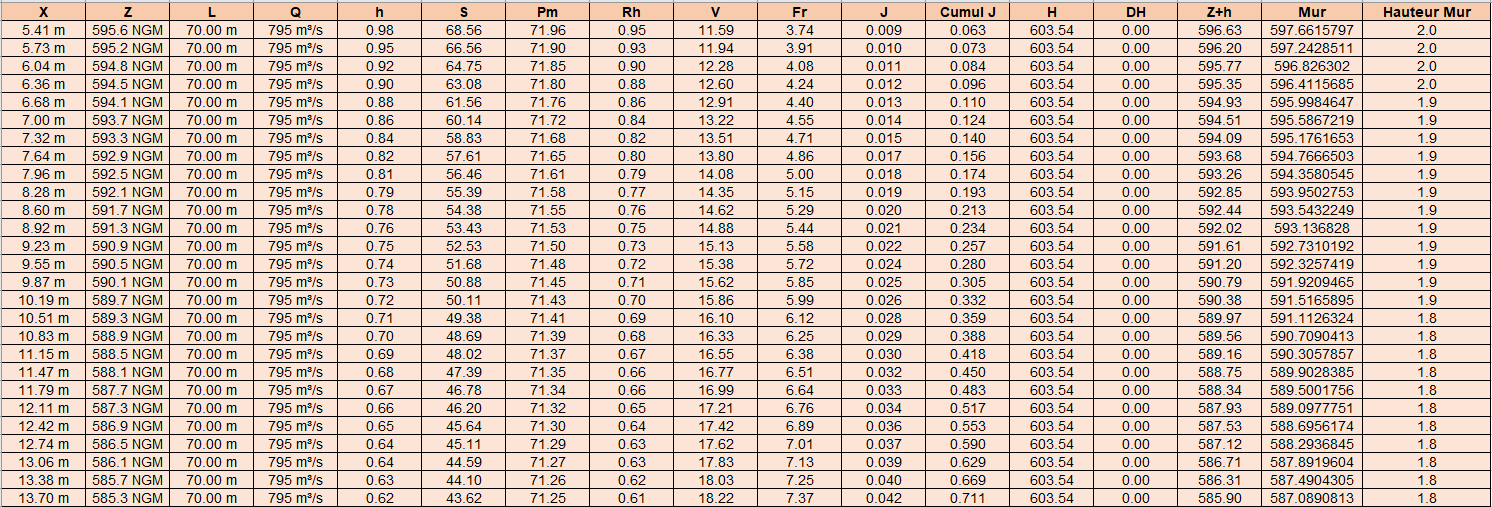
\includegraphics[width=\textwidth]{figures/tableau_mur_bajoyer_excel.png}
\end{table}

\paragraph{Comparaison des résultats Excel et HEC-RAS pour $Q_{1000}$}

Les deux approches appliquent la même formule de revanche USBR (équation \ref{eq:revanche}) pour $Q_{1000}$. Le tableau \ref{tab:comparaison_mur_excel_hecras} compare les hauteurs maximales obtenues.

\begin{table}[H]
    \centering
    \caption{Comparaison des hauteurs maximales de mur bajoyer, revanche incluse — calcul Excel et HEC-RAS ($Q_{1000} = 794{,}93$ m³/s)}
    \label{tab:comparaison_mur_excel_hecras}
    \begin{tabular}{|l|c|}
        \hline
        \textbf{Méthode} & \textbf{$H_{mur,max}$ (m)} \\
        \hline
        Calcul Excel section par section (colonne \og Hauteur Mur \fg{}, revanche incluse) & $2{,}00$ \\
        \hline
        Modélisation HEC-RAS : $H_{mur} = y_{max} + R_v = 2{,}00 + 0{,}83$ & $2{,}83$ \\
        \hline
        \textbf{Écart} $\Delta H$ & $\mathbf{0{,}83}$ \\
        \hline
    \end{tabular}
\end{table}

L'écart $\Delta H = 2{,}83 - 2{,}00 = 0{,}83$ m est égal à la revanche $R_v$ :

\[
R_v = 0{,}61 + 0{,}037 \times 4{,}81 \times 2{,}00^{1/3} = 0{,}83 \text{ m}
\]

La feuille de calcul Excel évalue la hauteur de mur section par section en intégrant la revanche à chaque pas via la même formule USBR, et retient le maximum sur l'ensemble du coursier, soit $H_{mur}^{\text{Excel}} = 2{,}00$ m. La modélisation HEC-RAS, quant à elle, construit la hauteur de mur à partir de la profondeur maximale enveloppe $y_{max} = 2{,}00$ m à laquelle elle ajoute explicitement $R_v = 0{,}83$ m, donnant $H_{mur}^{\text{HEC-RAS}} = 2{,}83$ m. C'est cette dernière valeur qui est retenue comme hauteur de référence pour le dimensionnement des murs bajoyers, car elle représente la condition la plus défavorable sur l'ensemble du coursier.

% SECTION : GÉOMÉTRIE DE LA CUILLÈRE
\section{Géométrie de la cuillère (saut de ski)}
\label{sec:geometrie_cuillere}

Le rôle de la cuillère du saut de ski est de dévier le jet d'eau issu du coursier vers le haut, afin de le projeter à distance du pied aval du barrage et de limiter ainsi le risque d'érosion régressive au contact direct de l'ouvrage. La géométrie de la cuillère du barrage Ahl Souss, présentée au chapitre \ref{chap:barrage}, est caractérisée par :
\begin{itemize}
    \item Une cote de calage du point bas de la cuillère $Z_c = 585{,}20$ NGM ;
    \item Un bec déviateur tracé selon un arc de cercle de rayon $R = 3$ m ;
    \item Un angle de sortie $\theta = 40°$ par rapport à l'horizontale.
\end{itemize}

D'un point de vue dimensionnel, le rayon $R$ de la cuillère doit être suffisant pour limiter la pression dynamique exercée sur le radier au point bas de la cuillère, où l'écoulement change brutalement de direction. L'USBR recommande de vérifier que le rapport entre le rayon de courbure et la profondeur d'eau au point de décollement du jet ($R/y_0$) reste supérieur à environ $4$, de manière à éviter les risques de décollement de la lame d'eau et de cavitation sur l'extrados de la cuillère \cite{usbr1987design}.

La profondeur $y_0$ et la vitesse $V_0$ au point de décollement du jet sont obtenues à partir de la dernière section calculée de la courbe de remous (section \ref{sec:courbe_remous}), à la cote $Z_0$ -- un point du profil de la cuillère situé légèrement au-dessus du point bas de calage $Z_c$. Le tableau \ref{tab:geometrie_cuillere} récapitule, pour chacun des trois débits laminés retenus, les conditions d'écoulement au point de décollement du jet ainsi que la vérification du critère $R/y_0$.

\begin{table}[H]
    \centering
    \caption{Conditions d'écoulement au point de décollement du jet et vérification géométrique}
    \label{tab:geometrie_cuillere}
    \begin{tabular}{|c|c|c|c|c|c|c|}
        \hline
        \textbf{Période de retour (ans)} & \textbf{$Q$ (m³/s)} & \textbf{$y_0$ (m)} & \textbf{$V_0$ (m/s)} & \textbf{$Z_0$ (m NGM)} & \textbf{$R/y_0$} & \textbf{Vérification} \\
        \hline
        10 & 160,74 & 0,128 & 17,89 & 583,91 & 23,37 & $R/y_0 > 4$ : OK \\
        \hline
        100 & 507,54 & 0,431 & 16,81 & 586,79 & 6,96 & $R/y_0 > 4$ : OK \\
        \hline
        1\,000 & 794,93 & 0,634 & 17,91 & 585,32 & 4,73 & $R/y_0 > 4$ : OK \\
        \hline
    \end{tabular}
\end{table}

Le critère $R/y_0 > 4$ est vérifié pour les trois débits laminés retenus, avec une marge qui se réduit logiquement lorsque le débit augmente, la profondeur $y_0$ croissant avec $Q$ alors que le rayon $R$ reste fixe. Le débit millénal $Q_{1000}$, le plus défavorable, présente la marge la plus faible ($R/y_0 \approx 4{,}7$), ce qui reste compatible avec le rayon $R = 3$ m retenu pour le bec déviateur.

\begin{figure}[H]
    \centering
    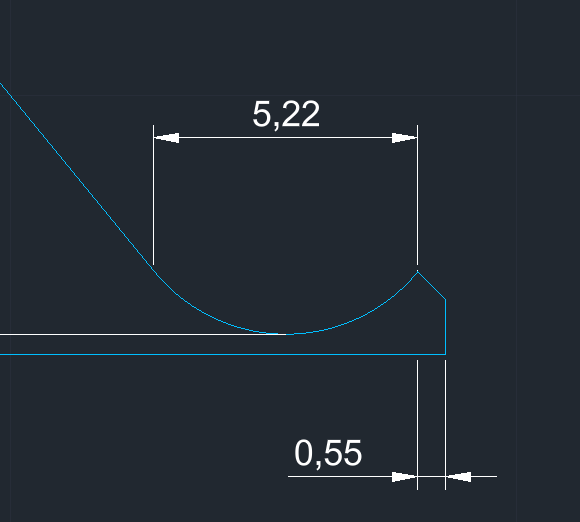
\includegraphics[width=0.65\textwidth]{figures/geometrie_cuillere.png}
    \caption{Géométrie de la cuillère et du bec déviateur du saut de ski.}
    \label{fig:geometrie_cuillere}
\end{figure}

% SECTION : DISTANCE D'IMPACT DU JET
\section{Distance d'impact du jet à l'aval}
\label{sec:distance_impact_jet}

À la sortie du bec déviateur, le jet d'eau quitte la cuillère avec une vitesse $V_0$ et un angle $\theta = 40°$ par rapport à l'horizontale, puis évolue en trajectoire libre jusqu'à son impact sur le terrain naturel ou le lit de l'oued. En prenant pour origine le point de sortie du bec déviateur, avec un axe $x$ horizontal orienté vers l'aval et un axe $z$ vertical orienté vers le haut, et en négligeant la résistance de l'air, la trajectoire du jet s'écrit \cite{usbr1987design} :

\begin{equation}
z(x) = x \tan\theta - \frac{g\,x^2}{2\,V_0^2 \cos^2\theta}
\label{eq:trajectoire_jet}
\end{equation}

Le point d'impact, situé à une dénivelée $\Delta Z = Z_0 - Z_{aval}$ en dessous du point de décollement du jet (avec $Z_{aval} = 579{,}50$ NGM la cote du radier du bassin de dissipation, tableau \ref{tab:donnees_base}), est obtenu en posant $z(x) = -\Delta Z$ dans l'équation \ref{eq:trajectoire_jet}, ce qui conduit, après résolution de l'équation du second degré en $x$, à la distance d'impact $L_x$ :

\begin{equation}
L_x = V_0 \cos\theta \cdot \frac{V_0 \sin\theta + \sqrt{(V_0 \sin\theta)^2 + 2 g \Delta Z}}{g}
\label{eq:distance_impact}
\end{equation}

La vitesse $V_0$ et la cote $Z_0$ au point de décollement du jet sont issues du tableau \ref{tab:geometrie_cuillere} (section \ref{sec:geometrie_cuillere}). Le tableau \ref{tab:distance_impact} présente la distance d'impact $L_x$ obtenue pour chacun des trois débits laminés retenus.

\begin{table}[H]
    \centering
    \caption{Distance d'impact du jet pour les débits laminés retenus}
    \label{tab:distance_impact}
    \begin{tabular}{|c|c|c|c|c|}
        \hline
        \textbf{Période de retour (ans)} & \textbf{$Q$ (m³/s)} & \textbf{$V_0$ (m/s)} & \textbf{$\Delta Z$ (m)} & \textbf{$L_x$ (m)} \\
        \hline
        10 & 160,74 & 17,89 & 4,41 & 36,72 \\
        \hline
        100 & 507,54 & 16,81 & 7,29 & 35,36 \\
        \hline
        1\,000 & 794,93 & 17,91 & 5,82 & 38,07 \\
        \hline
    \end{tabular}
\end{table}

Les valeurs de $L_x$ restent comprises entre 35 et 38 m pour les trois débits étudiés : les variations de $V_0$ et de $\Delta Z$ se compensent partiellement, sans tendance strictement monotone.

La figure \ref{fig:trajectoire_jet} présente la trajectoire du jet obtenue par la modélisation sous tableur Excel pour le débit millénaire $Q_{1000} = 794{,}93$ m³/s, avec les mêmes paramètres que ceux du tableau \ref{tab:distance_impact} (talus aval $= 0{,}8\,\mathrm{H}/1\,\mathrm{V}$, longueur de passe $= 70$ m, PHE $= 603{,}1$ m NGM, PHE\,aval $= 574$ m NGM).

\begin{figure}[H]
    \centering
    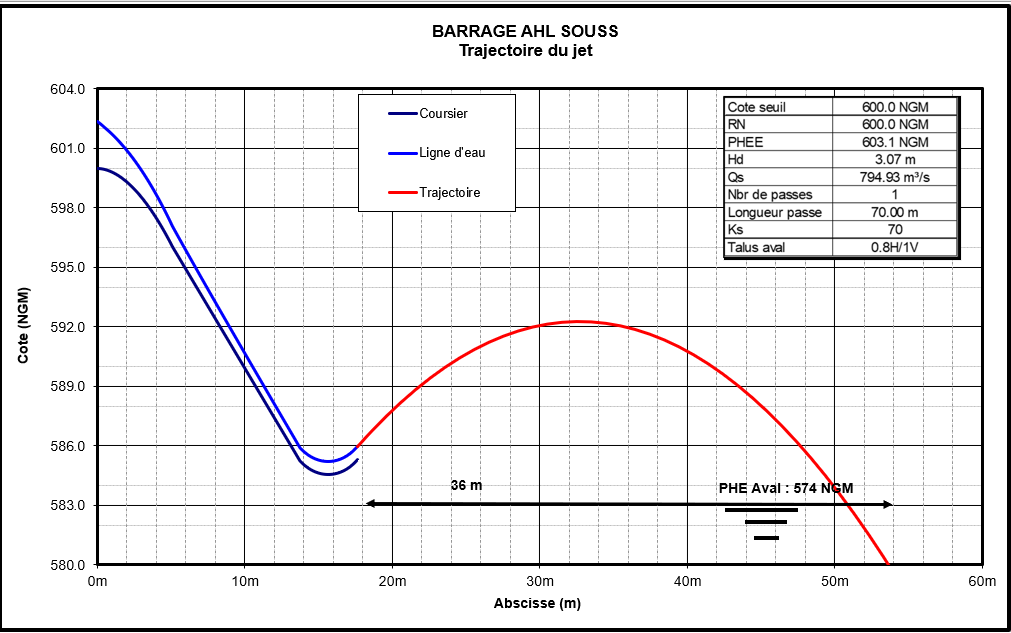
\includegraphics[width=0.92\textwidth]{figures/trajectoire_jet.png}
    \caption{Trajectoire du jet issu de la cuillère saut de ski — Barrage Ahl Souss, $Q_{1000} = 794{,}93$ m³/s (modélisation Excel)}
    \label{fig:trajectoire_jet}
\end{figure}

Le graphe Excel indique une distance d'impact $L_x^{\mathrm{Excel}} \approx 36$ m pour $Q_{1000}$, à comparer avec la valeur analytique $L_x^{\mathrm{calc}} = 38{,}07$ m issue de l'équation \ref{eq:distance_impact}. L'écart entre les deux estimations est de l'ordre de \textbf{5,4\,\%}, ce qui est tout à fait acceptable compte tenu des hypothèses simplificatrices de la trajectoire parabolique (résistance de l'air négligée, angle de décollement fixé à $40°$). Les deux approches confirment que le jet retombe à une distance d'environ 36 à 38 m du pied de la cuillère, bien au-delà du pied aval du barrage, et que sa trajectoire reste compatible avec l'emprise du bassin de dissipation projeté (chapitre \ref{chap:barrage}).

% SECTION : AFFOUILLEMENT
\section{Évaluation de l'affouillement à l'aval du barrage}
\label{sec:affouillement}

L'impact du jet issu du saut de ski sur le lit de l'oued provoque, à long terme, le développement d'une fosse d'érosion (ou fosse d'affouillement) dont la profondeur conditionne la stabilité du pied aval de l'ouvrage et des éventuels dispositifs de protection. Afin d'encadrer cette profondeur, quatre formules empiriques classiques ont été appliquées, chacune basée sur le débit unitaire $q = Q/L$ et une hauteur de chute caractéristique :

\begin{itemize}
    \item $H$ : dénivelée entre la cote PHE et la cote de départ du jet $Z_0$ (cuillère), soit $H = \mathrm{PHE} - Z_0$ ;
    \item $h^*$ : charge totale de chute entre la cote PHE et la cote du lit aval (PHE aval), soit $h^* = \mathrm{PHE} - \mathrm{PHE_{aval}}$.
\end{itemize}

\noindent\textbf{Formule de Veronese} \cite{usbr1987design} :
\begin{equation}
D = 1{,}90 \; q^{0,54} \; H^{0,225}
\label{eq:affouillement_veronese}
\end{equation}

\noindent\textbf{Formule de Damle} :
\begin{equation}
D = 0{,}65 \; q^{0,50} \; (h^*)^{0,50}
\label{eq:affouillement_damle}
\end{equation}

\noindent\textbf{Formule de Martins} :
\begin{equation}
D = 1{,}5 \; q^{0,60} \; H^{0,10}
\label{eq:affouillement_martins}
\end{equation}

\noindent\textbf{Formule de Chian} :
\begin{equation}
D = 1{,}18 \; q^{0,51} \; H^{0,235}
\label{eq:affouillement_chian}
\end{equation}

\noindent où $D$ est la profondeur d'affouillement mesurée sous le niveau du lit aval (m) et $q$ le débit unitaire (m²/s).

\medskip
Les calculs ont été réalisés pour les trois débits de crue retenus. Pour chaque débit, les paramètres $H$ (dénivelée PHE\,--\,départ du jet) et $h^*$ (dénivelée PHE\,--\,PHE\,aval) sont issus du bilan hydraulique du coursier. La cote de fond de fosse est obtenue par : cote\,=\,PHE\,aval\,$- D$, la PHE aval commune étant de 596,19 m NGM.

\subsubsection*{Débit décennal --- $Q_{10} = 161$ m³/s}

\begin{figure}[H]
    \centering
    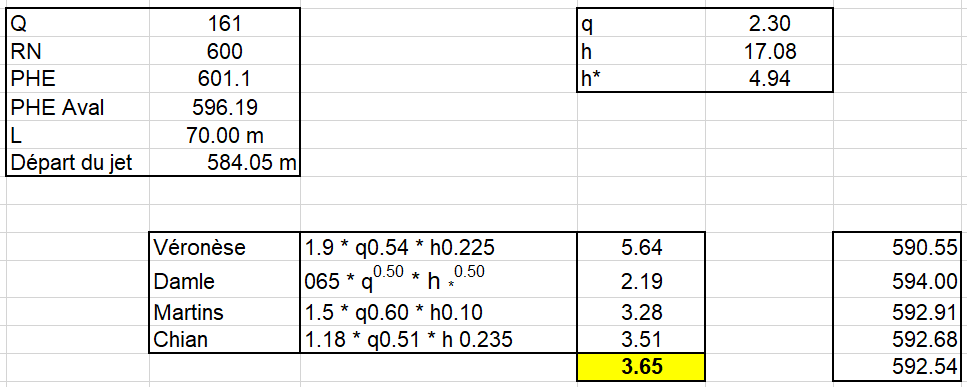
\includegraphics[width=\textwidth]{figures/fosse_q10.png}
    \caption{Calcul de la profondeur d'affouillement pour $Q_{10} = 161$ m³/s ($q = 2{,}30$ m²/s, $H = 17{,}08$ m, $h^* = 4{,}94$ m) — résultats des quatre formules empiriques}
    \label{fig:fosse_q10}
\end{figure}

Pour le débit décennal ($Q_{10} = 161$ m³/s, $q = 2{,}30$ m²/s), les profondeurs d'affouillement calculées varient de 2,19 m (Damle) à 5,64 m (Veronese). La valeur moyenne est $D_{10} = 3{,}65$ m, correspondant à une cote de fond de fosse de $596{,}19 - 3{,}65 = \mathbf{592{,}54}$ m NGM. La faiblesse du débit unitaire pour ce scénario explique les profondeurs modestes obtenues par l'ensemble des formules.

\subsubsection*{Débit centennal --- $Q_{100} = 508$ m³/s}

\begin{figure}[H]
    \centering
    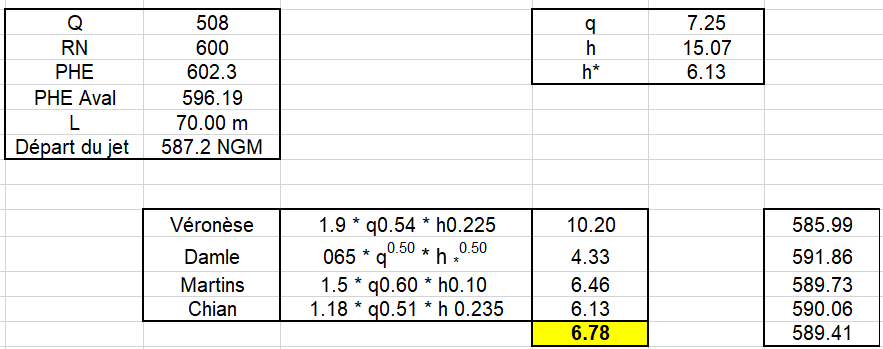
\includegraphics[width=\textwidth]{figures/fosse_q100.png}
    \caption{Calcul de la profondeur d'affouillement pour $Q_{100} = 508$ m³/s ($q = 7{,}25$ m²/s, $H = 15{,}07$ m, $h^* = 6{,}13$ m) — résultats des quatre formules empiriques}
    \label{fig:fosse_q100}
\end{figure}

Pour le débit centennal ($Q_{100} = 508$ m³/s, $q = 7{,}25$ m²/s), les profondeurs obtenues s'étendent de 4,33 m (Damle) à 10,20 m (Veronese). La valeur moyenne est $D_{100} = 6{,}78$ m, pour une cote de fond de fosse de $596{,}19 - 6{,}78 = \mathbf{589{,}41}$ m NGM. La nette augmentation du débit unitaire par rapport à $Q_{10}$ se traduit par un creusement sensiblement plus important.

\subsubsection*{Débit millénaire --- $Q_{1000} = 795$ m³/s}

\begin{figure}[H]
    \centering
    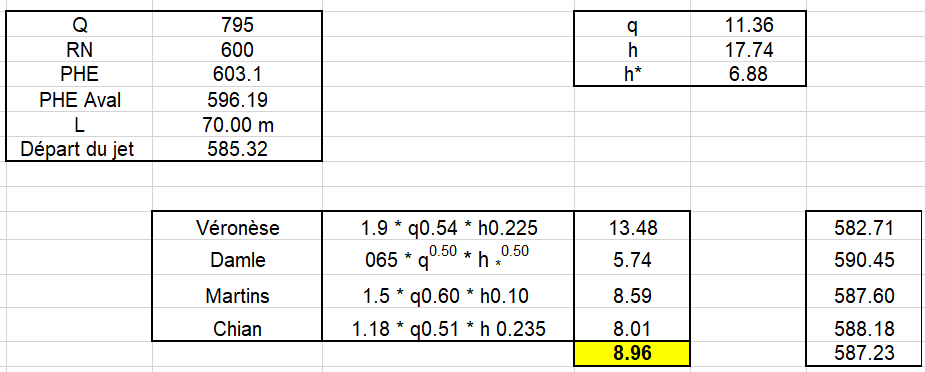
\includegraphics[width=\textwidth]{figures/fosse_q1000.png}
    \caption{Calcul de la profondeur d'affouillement pour $Q_{1000} = 795$ m³/s ($q = 11{,}36$ m²/s, $H = 17{,}74$ m, $h^* = 6{,}88$ m) — résultats des quatre formules empiriques}
    \label{fig:fosse_q1000}
\end{figure}

Pour le débit millénaire ($Q_{1000} = 795$ m³/s, $q = 11{,}36$ m²/s), scénario le plus sévère, les profondeurs calculées s'étalent de 5,74 m (Damle) à 13,48 m (Veronese). La valeur moyenne est $D_{1000} = 8{,}96$ m, soit une cote de fond de fosse de $596{,}19 - 8{,}96 = \mathbf{587{,}23}$ m NGM.

\medskip
Le tableau \ref{tab:affouillement} récapitule l'ensemble des résultats pour les trois débits étudiés :

\begin{table}[H]
    \centering
    \caption{Profondeur d'affouillement $D$ (m) et cote de fond de fosse (m NGM) — comparaison des quatre formules empiriques pour les trois débits de crue (PHE\,aval $= 596{,}19$ m NGM)}
    \label{tab:affouillement}
    \resizebox{\textwidth}{!}{%
    \begin{tabular}{|l|c|c|c|c|c|c|}
        \hline
        \textbf{Formule} & \multicolumn{2}{c|}{$Q_{10} = 161$ m³/s} & \multicolumn{2}{c|}{$Q_{100} = 508$ m³/s} & \multicolumn{2}{c|}{$Q_{1000} = 795$ m³/s} \\
        \hline
        & $D$ (m) & Cote (m NGM) & $D$ (m) & Cote (m NGM) & $D$ (m) & Cote (m NGM) \\
        \hline
        Veronese  & 5,64 & 590,55 & 10,20 & 585,99 & 13,48 & 582,71 \\
        \hline
        Damle     & 2,19 & 594,00 &  4,33 & 591,86 &  5,74 & 590,45 \\
        \hline
        Martins   & 3,28 & 592,91 &  6,46 & 589,73 &  8,59 & 587,60 \\
        \hline
        Chian     & 3,51 & 592,68 &  6,13 & 590,06 &  8,01 & 588,18 \\
        \hline
        \textbf{Moyenne} & \textbf{3,65} & \textbf{592,54} & \textbf{6,78} & \textbf{589,41} & \textbf{8,96} & \textbf{587,23} \\
        \hline
    \end{tabular}}
\end{table}

La profondeur d'affouillement croît avec le débit de crue, passant d'une moyenne de 3,65 m pour $Q_{10}$ à 8,96 m pour $Q_{1000}$. Pour le scénario dimensionnant ($Q_{1000} = 795$ m³/s), la valeur retenue est $D = 8{,}96$ m, correspondant à une cote de fond de fosse de \textbf{587,23 m NGM}. Cette cote reste nettement supérieure aux fondations du barrage, confirmant l'absence de risque direct d'affouillement sur les fondations ; le cas échéant, une protection complémentaire (enrochement, radier aval) pourra être dimensionnée en référence à cette valeur.

% SECTION : SYNTHÈSE DES RÉSULTATS THÉORIQUES
\section{Synthèse des résultats théoriques}
\label{sec:synthese_resultats_theoriques}

Les sections précédentes ont permis d'établir, pour chacun des trois débits laminés étudiés, l'ensemble des grandeurs hydrauliques caractéristiques du fonctionnement de l'évacuateur de crues : charge sur le seuil, profondeur et vitesse d'écoulement le long du coursier, hauteur des murs bajoyers, conditions d'écoulement au niveau de la cuillère, distance d'impact du jet et profondeur d'affouillement. Le tableau \ref{tab:synthese_theorique} regroupe l'ensemble de ces résultats théoriques.

\begin{table}[H]
    \centering
    \caption{Synthèse des résultats théoriques pour les débits laminés retenus}
    \label{tab:synthese_theorique}
    \resizebox{\textwidth}{!}{%
    \begin{tabular}{|c|c|c|c|c|c|c|c|}
        \hline
        \textbf{$T$ (ans)} & \textbf{$Q$ (m³/s)} & \textbf{$H$ (m)} & \textbf{$y_{max}$ coursier (m)} & \textbf{$H_{mur}$ (m)} & \textbf{$V_0$ cuillère (m/s)} & \textbf{$L_x$ (m)} & \textbf{$D$ (m)} \\
        \hline
        10 & 160,74 & 1,13 & 1,10 & 1,82 & 17,89 & 36,72 & 3,65 \\
        \hline
        100 & 507,54 & 2,32 & 1,60 & 2,39 & 16,81 & 35,36 & 6,78 \\
        \hline
        1\,000 & 794,93 & 3,07 & 2,00 & 2,83 & 17,91 & 38,07 & 8,96 \\
        \hline
    \end{tabular}}
\end{table}

Ce tableau récapitulatif constitue la base de comparaison de référence pour l'analyse des résultats de la modélisation numérique sous OpenFOAM, présentée au chapitre \ref{chap:resultats_simulation} (section \ref{sec:comparaison_theorie_numerique}). Pour chaque débit de crue simulé, les grandeurs obtenues numériquement (charge sur le seuil, hauteur d'eau le long du coursier, trajectoire et distance d'impact du jet) seront confrontées aux valeurs théoriques de ce tableau, afin d'évaluer la cohérence du dimensionnement existant et d'identifier d'éventuels écarts entre l'approche 1D/empirique et l'approche tridimensionnelle.
